\documentclass{article}
\usepackage[utf8]{inputenc}
\usepackage[margin=1in]{geometry}
\usepackage{graphicx}
\usepackage{natbib}
\usepackage{enumitem}
\usepackage{array}
\usepackage{gensymb}
\usepackage{indentfirst}
\graphicspath{ {Images/} }
\usepackage{float}
\usepackage[table,xcdraw]{xcolor}
\usepackage{amsmath}
\usepackage{adjustbox}
\usepackage{url}

\title{Physics 111A Lab 12:\\ Instrument Digital Auto-Tuner: \\Trick Yourself Into Thinking You Are Good At Playing Instruments}
\author{Joshua Levy\\Lab Partner- Alex Chuang }
\date{December 11th, 2016}



\begin{document}

\maketitle

\begin{center}
    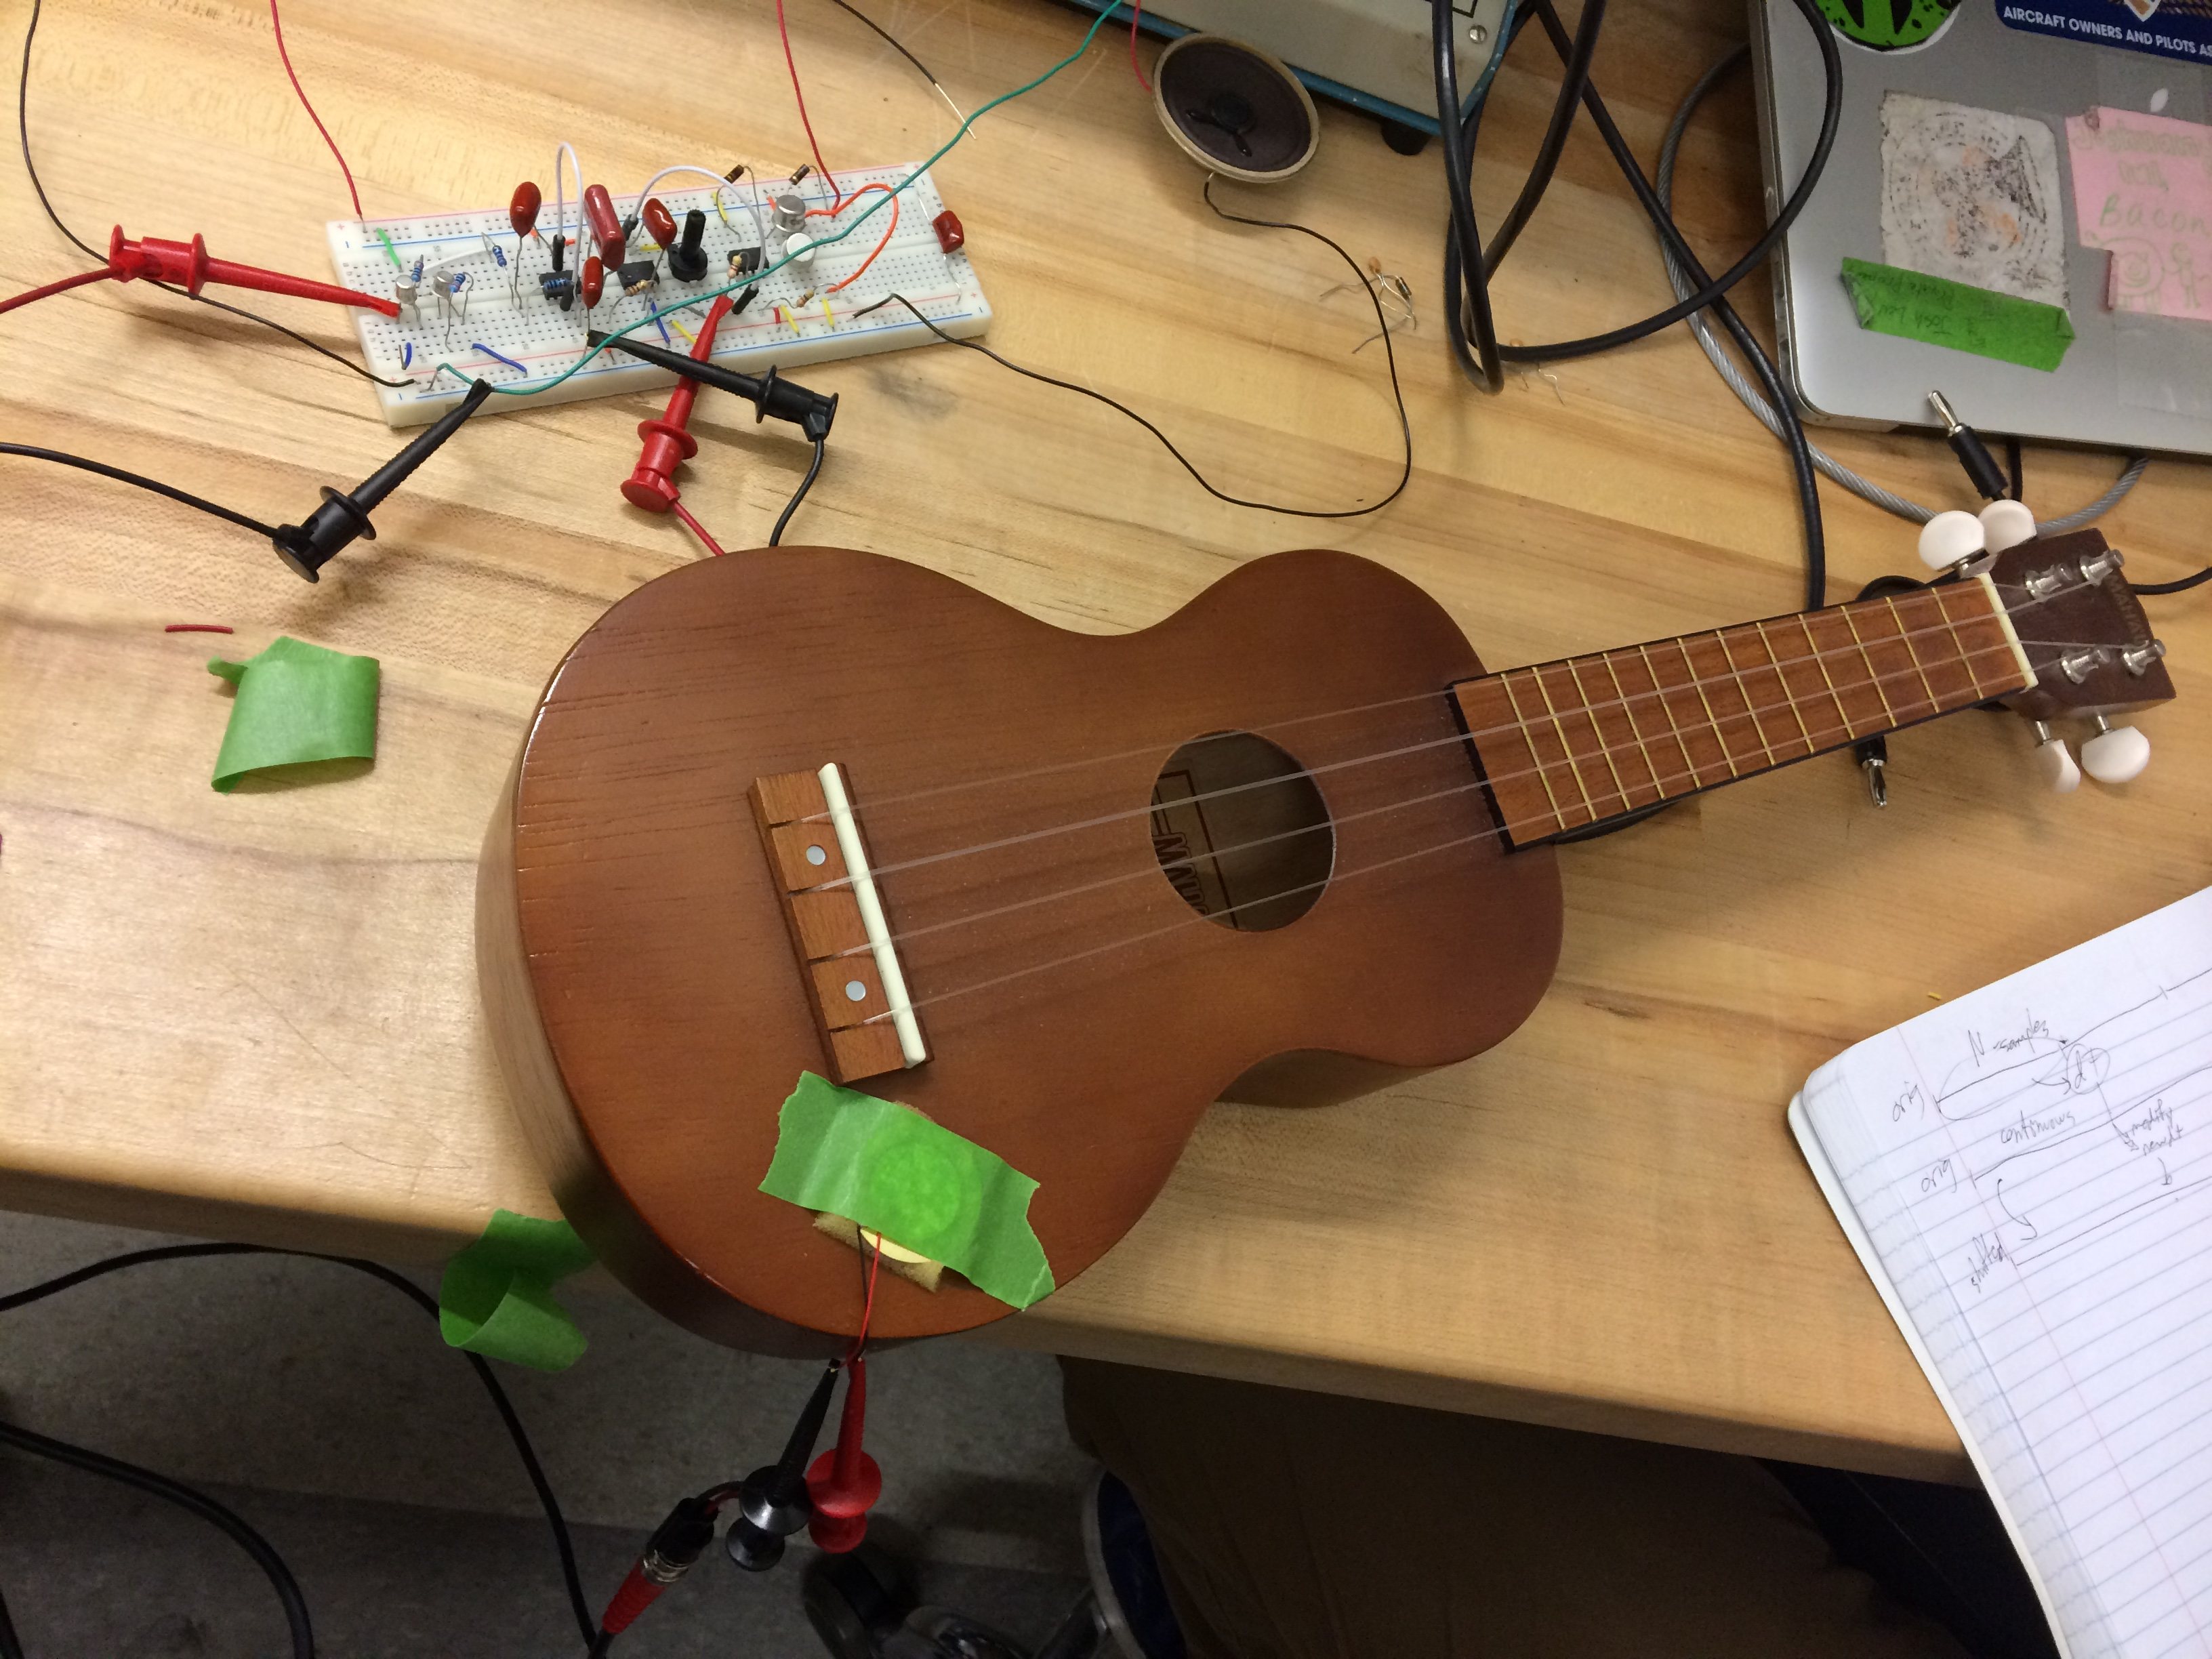
\includegraphics[scale = 0.07]{Auto1.JPG}
\end{center}

\section{Abstract}
    My partner and I built a circuit that converts mechanical vibrations of any instrument into electrical signals and shifts the frequency of a signal to a desired frequency. We manipulated signal voltage offsets, noise, and volume, and sent the signal to both an analog speaker to be played and to a computer analog input for LabView/MatLab analysis. We were able to shift the signal frequency to the closest musical note and to user-specified frequencies. We also converted series of played notes at arbitrary frequencies into a known song. We explored piezoelectric effects, signal processing techniques, and how to auto-detect signals.\\\begin{table}[H]
\centering
\caption{Grading Matrix}
\label{my-label}
\begin{tabular}{|l|l|l|}
\hline
Introduction &  & 20 \\ \hline
Diagrams &  & 20 \\ \hline
Description &  & 40 \\ \hline
Level of Functioning &  & 40 \\ \hline
Design Creativity &  & 40 \\ \hline
Measurements &  & 10 \\ \hline
Conclusions &  & 10 \\ \hline
References &  & 5 \\ \hline
Instructor Arb Adjust &  &  \\ \hline
Total &  & 185 \\ \hline
\end{tabular}
\end{table} \newpage
\section{Introduction}
    My partner and I designed a circuit that would use piezoelectric elements as a transducer to convert mechanical vibrations of a playing instrument into electrical signals. These electrical signals would pass through various mechanisms in our circuit that would reduce noise, eliminate any DC offset, filter out unwanted high frequency signals, and control for volume using a variable resistor in an inverting op amp amplifier. Our circuit then splits this signal and sends some of it to an analog speaker system via a push-pull mechanism, and the other part of the signal towards the analog input of a computer to be converted to digital for digital signal processing. The defining feature of our final project is the digital manipulations/processing of the signal, which will allow you to better tune your instrument and play songs like you are a very talented musician (process to be described later in this section). 
    \\\indent The main aims of our final project were: 
    \begin{enumerate}
        \item To be able to convert mechanical vibrations of an instrument into electrical signals to be manipulated.
        \item To produce frequency shifts in this electrical signal. 
        \item To output the manipulated and original signal over computer and analog speakers respectively (computer output because of signal processing and analog output because of desire for continuous amplification of instrument sound).
    \end{enumerate}
    \indent Some underlying motivations for this project were:
    \begin{enumerate}
        \item Practice signal acquisition and processing.
        \item Become more comfortable with working in the frequency domain of data, which is very important in audio/sound engineering; other applications towards astronomy, and other important fields.
        \item Learn more about the physics behind piezo electrics.
        \item Pretend to be good at playing various instruments (eg. play random notes and have them all be shifted to the notes of a real song) and to have something that can help us tune any instrument or make the output of it sound better.
    \end{enumerate}
    \indent The aims could be accomplished by utilizing a transducer (piezo elements) to convert the mechanical vibrations to electrical signals, performing digital manipulations (via LabView and MatLab) of the data to perform "real-time" and post-processing "Song Shifter" frequency shifting of the signal's frequency spectrum, and the signals were outputted either through analog speakers or through computer speakers. We would also need to establish a trigger threshold of what it means to play a note to know when to begin recording/manipulating the signal data. For this project, we chose to only play one individual string at a time instead of chords in order to reduce some computational complexities. The algorithms employed, "real-time" analysis and "Song-Shifter" would shift the signal's frequency either to any user specified frequency, to the nearest note on a musical scale (to give you information on how to "tune" the instrument), and to shift a series of notes played with an arbitrary rhythm to match the tone and rhythm of any desired song you wish to play. \\\indent As you will see throughout the lab, some complexities do occur, and due to the nontrivial nature of real-time signal analysis, some compromises were made that still produce some pretty telling results. We expect any signals that were digitally manipulated would have proper frequency shifts to specified frequencies and fewer distortions in our final signal after manipulation would strengthen our conclusions.
    
    
\section{Description of Circuit}
    \subsection{Block Diagram}
        \begin{figure}[H]
            \centering
            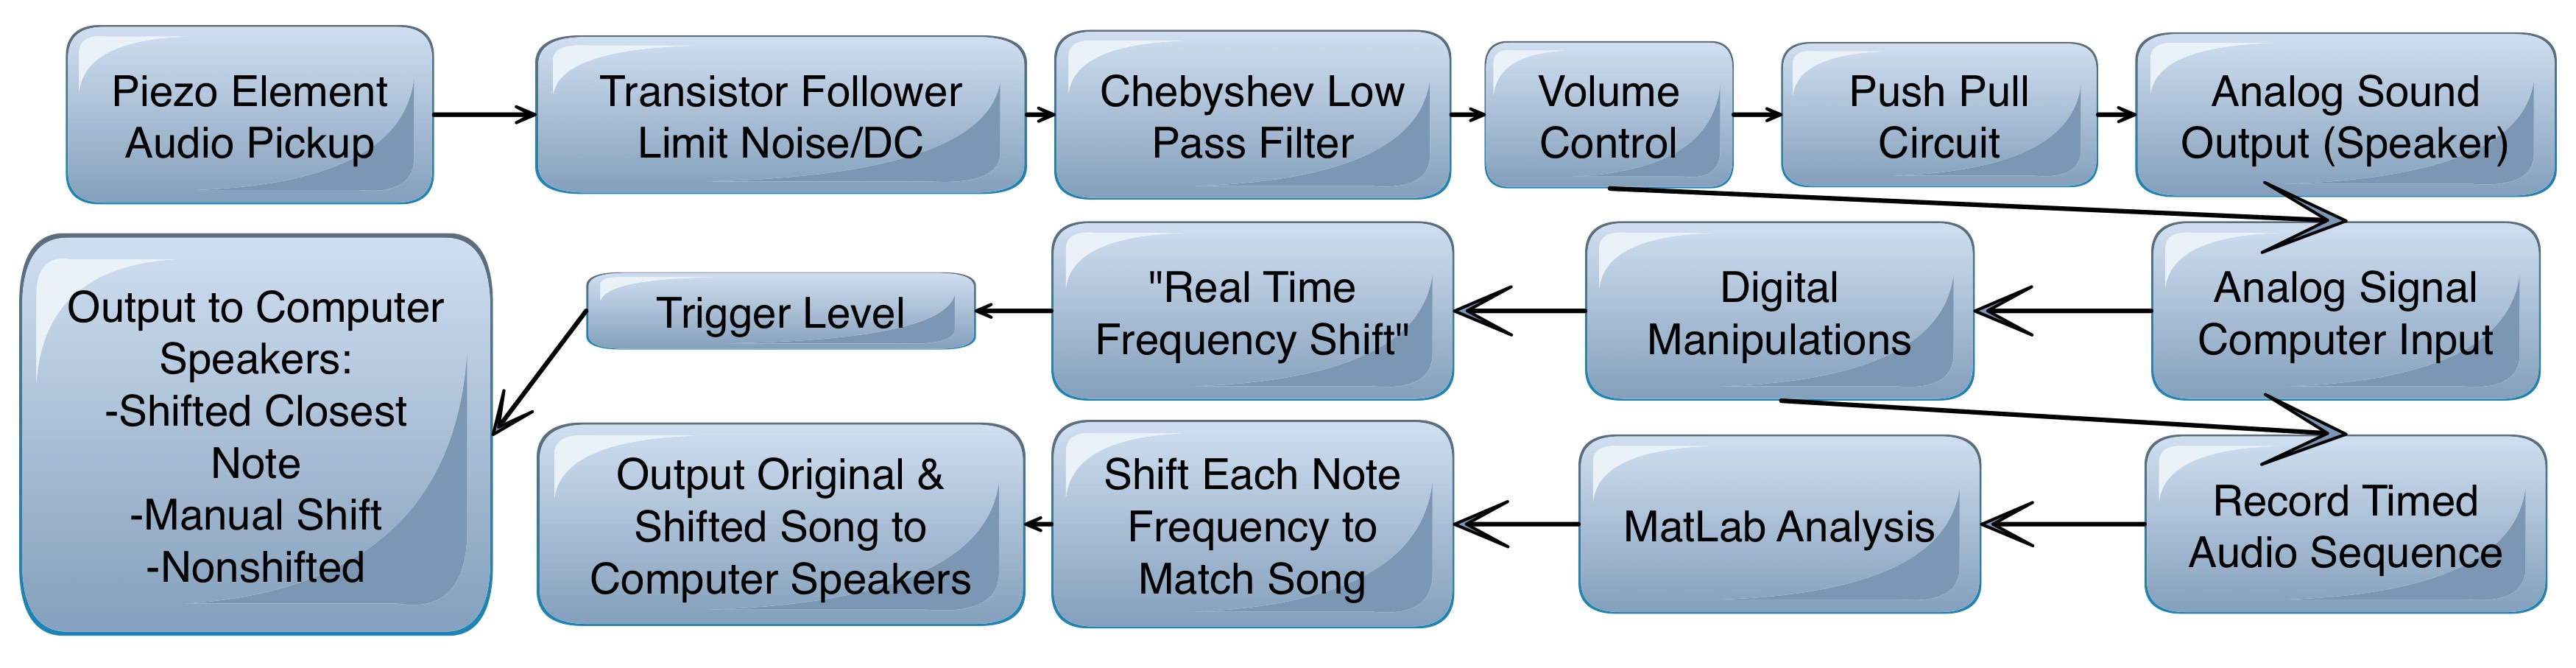
\includegraphics[scale = 0.13]{finalBlockDiagram.jpg}
            \caption{Block Diagram}
            \label{fig:my_label}
        \end{figure}
    \subsection{Circuit Diagram}
        \begin{figure}[H]
            \centering
            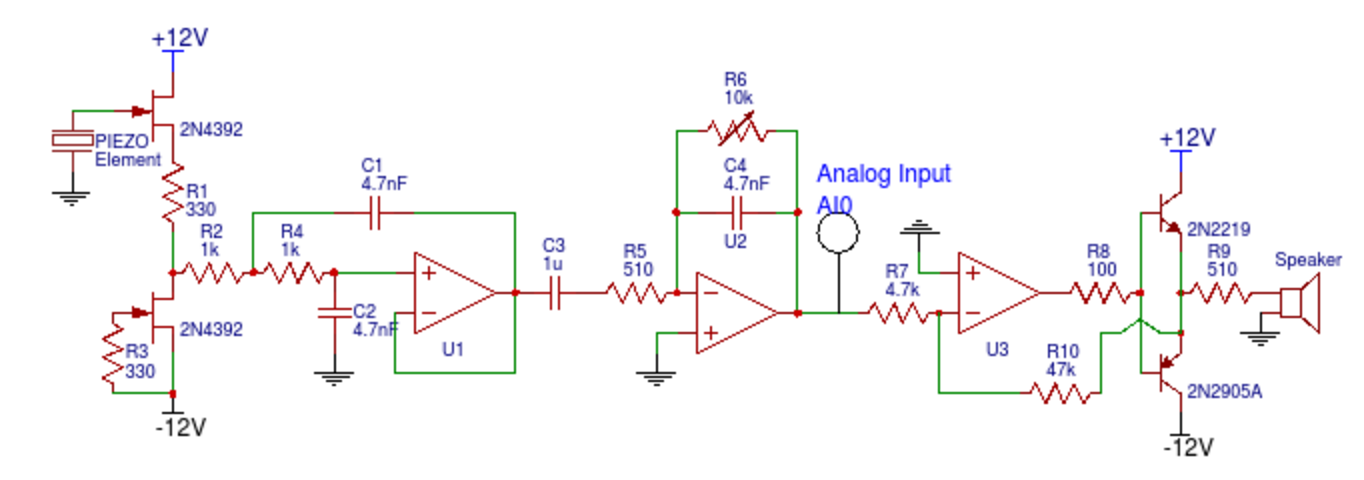
\includegraphics[scale = 0.6]{circuitFinal.png}
            \caption{Circuit Diagram}
            \label{fig:my_label}
        \end{figure}
    \subsection{Purpose and Operation of All the Major Components: Circuit and Digital Manipulations (Computer Analysis)}
    \begin{itemize}
        \item Piezoelectric element: We taped this element onto the instrument in order to turn acoustic vibrations into an electrical voltage signal; the description of how this element works will be covered in the theory section. The piezo electric element has a 27mm diameter plate made out of brass with a 20mm diameter ceramic element. Please note only one string/note is played at a time. \cite{piezo1}
        \item The improved JFET follower II from lab 4 was used to impedance match with the piezo electric element to maximize power and amplify the current to drive the circuit and largely eliminate any DC offset in the electrical signal. A pair of 3.3k resistors were used to control the current entering the circuit part and the symmetry of the follower helped with reducing the offset (slight offset still exists because of any asymmetries in the circuit). \cite{lab4}
        \item Op amp Low Pass Filter- this was a Chebyshev Filter with Salley Key Topology with a rolloff frequency of about 40kHz. The rolloff frequency is $f_r = \frac{1}{\sqrt{R_2*C_1*R_4*C_2}}$, both resistor values were about 1k, and the capacitors used had capacitance of 4.7nF. We used this element to reduce any possible sources of high frequency noise (tapping for instance) and harmonics, and also to limit the frequency of data we're digitally manipulating. It has a sharp rolloff. \cite{wiki1}
        \item Volume control element: inverting op amp amplifier with feedback capacitor (to block high frequency oscillations) in parallel with feedback variable resistor (10k potentiometer). The variable resistor adjusts the gain of signal passing through allowing you to change the volume gain of the signal passing through from 0 to much larger than 1 values. The input capacitor for $V_-$ is used to completely block any DC offset.
        \item A wire was connected between volume control and the DAC card for digital to analog conversion. This was an analog Input (AI0) to computer for digital manipulation and output the manipulated digitized signal over computer speakers. Digital manipulations include (these points will be discussed further in the theory section):
        \begin{itemize}
            \item Song Shifting: Use a Labview program to take in a signal over a set period of time at 100k sampling rate. Then import the Labview data into MatLab. Use a matlab script to separate the signal into individual notes in the time-domain. Use a phase vocoder technique that utilizes fast fourier transforms (FFTs) to stretch each note's time domain data while preserving the frequency information. Then resample the data to return the time domain back to the time length of the note and also causing shift in the frequency of the note to frequency specified by the desired song.
            \item "Real Time" Frequency Shift- Loops continuously through a LabView program that collects 100ms samples of data at 100k sampling rate (large sampling rate so that we could sample above the Nyquist frequency 40kHz and to improve signal quality). Once the amplitude of the sample passes a certain voltage threshold specified by the user, the program performs digital manipulations of the data. The user can specify to shift the fundamental frequency of the data (and the all of the frequencies in the sample because only one note is being played at a time, i.e. no chords) of the sample to a frequency that is manually defined or to the closest note on a musical scale containing information 8 octaves of musical note letters and their corresponding frequencies; the latter is used for tuning purposes. The frequency shift is done by changing the dt (time in between each sample point) of the time-domain data of the signal to match that of the shifted frequency. The fast fourier transforms of the shifted data and original signal data are displayed on waveform graphs nearby their time domain graphs and information is conveyed to the user about how far off they were from the frequency and note (in Hz). This is not exactly real-time data because samples were taken in 100ms chunks, processing time caused the program to increase buffering time, and the total time of the shifted frequency signal sample changed.
        \end{itemize}
        \item Push-Pull Circuit: To prepare signal for speaker output by decreasing distortions in the speaker output by bypassing the current limitations of op amps from previous stages and delivering the proper amount of power to be dissipated by the speaker.
        \item Analog Speaker: Will play filtered original raw signal audio continuously to boost sound coming from instrument.
    \end{itemize}

\section{Theory and Elaboration on Signal Processing}
    \subsection{Piezo Electric Element Information}
    The piezo electric element we used in our circuit is made out of brass and ceramics. The piezoelectric effect in materials (which allows mechanical stress in a material to be transduced to an electrical signal is related to the use of electric dipole moments $\vec{p_i}$ in solids and their corresponding polarization $\vec{P}$, which is the dipole volume density $\sum_i{\frac{\vec{p_i}}{Volume}}$. Dipoles near each other tend to be aligned, and strong external electric fields can aid in this alignment. The polarization of a material can change when a mechanical stress is applied because the stress can reorient the molecular dipole moments or reconfigure the surrounding that will in turn induce different dipole moments. Thus, mechanical stress will cause changes in the localized polarization vector of the material in both direction and strength. Because the polarization can be represented as a separation of charge densities, we see that a material that has undergone a change in polarization will undergo a change in surface charge densities. Changes in surface charge densities will generate corresponding differences in electric fields, which result in changes in electric potentials over time, which is essentially our signal. The positive lead from our piezo electric element is connected to the ceramic piece and the negative lead is connected to the brass piece, and we see that these boundary changes in electric fields via changes in polarization due to mechanical stress (also depending on the polarization's orientation and molecular/crystal symmetry in the material) will generate a signal that will conduct to our circuit to be measured.\\ From a mathematical standpoint, we see that in a linear dielectric material, which is like the ceramic piece used on the :
    \begin{equation}
        \vec{D} = \epsilon \vec{E}, \vec{P} = \epsilon_0 \chi_e \vec{E}
    \end{equation}
    where $\vec{D}$ is the electric displacement, $\epsilon$ is the permittivity, and $\chi_e$ is the electric susceptibility of the material. We see that mechanical stress, represented by Hooke's law:
    \begin{equation}
        \vec{S} = s \vec{T}
    \end{equation}
    where $\vec{S}$ is the strain of the material, $\vec{T}$ is the applied mechanical stress and s is the flexibility of the material. And we see that we can couple the two equations to demonstrate the piezoelectric effect: 
    \begin{equation}
        \vec{D} = \delta \vec{T} + \epsilon \vec{E}
    \end{equation} 
    where $\delta$ is the direct piezo electric effect. The generated signal V is related to the electric field of the coupled equation by:
    \begin{equation}
        \vec{E} = -\bigtriangledown V
    \end{equation}
    Please see Figure 4 of the appendix for a visual description of what is generating this signal via the piezo electric effect. \cite{wiki2}
    \cite{piezo1}
    \subsection{Signal Processing and Post-Analysis Methods}
        Two different methods were used to shift the frequency of the signal/incoming note:
        \begin{enumerate}
            \item "Real Time" Shifter via LabView Analysis- As we mentioned previously, the real time shifter is not actually real time, but it takes continuously looped 100ms samples of the signal and shifts the fundamental/peak frequency (and all of the frequencies in the frequency spectrum) of the sample to a new specified frequency (the new specified frequency is either to the closest note specified by musical scales or a manually specified frequency; denote as $f_s$). The sample's fundamental frequency (denote as $f_f$) was found by taking the FFT of the sample and finding the frequency of the maximum amplitude value of the FFT. The $f_f$ scales to the $f_s$ by $f'= \frac{f_s}{f_f}$, so we can horizontally stretch/compress the frequency domain of the FFT by:
            \begin{equation}
                f_{new} = f_{old} * f'
            \end{equation}
            and inverse FFT (iFFT) back to the time domain. However, this is essentially equivalent to changing the dt, the amount of time between each sample point in the time domain of the signal, thus generating a horizontal time stretch/compression in the time domain. LabView has waveform data types that are specified by dt, the time between each data point, and Y, the amplitude data of the time-domain waveform. We maintained the Y-values of the waveform, but modified the dt by specifying a new dt':
            \begin{equation}
                dt' = \frac{dt}{f'} = \frac{dt*f_f}{f_s}
            \end{equation}
            However, the total time of the sample is also changed to N (number of sample points) * dt', so the amount of time a sample is played for is not constant. This is fixed via the phase vocoder method.
            \item Post-Processing Song Shifter Phase Vocoder Method- A particular rhythm with arbitrary notes were played on the instrument, recorded on Labview, and sent to MatLab for analysis. The notes were broken up into via a method that will be described. Now we consider one note, which typically is modelled by a linear superposition of harmonic sine waves with a modulating exponential decay function, for instance:
            \begin{equation}
                V(t) = exp(-kt)\sum_n A_n sin(2\pi f_f nt)
            \end{equation}
            where k is the decay factor. We aimed to maintain the same total time T for the note played, but replace $f_f$ with $f_s$, the note specified by the note in the song to be played. First, we stretch the total time of the sample out by the relationship:
            \begin{equation}
                T' = T*f' = T*\frac{f_s}{f_f}
            \end{equation}
            However, the stretching was done using a phase vocoder process (see Figure 5), we were able to increase the total time and data points in the sample/note, but preserved the frequency information of the original sample. This was done by separating breaking the time-domain sample points up into a series of overlapping windows (see Figure 5a). These windows are each horizontally translated rightward (not stretching data point spacing; also, windows could shift leftwards depending on if f' $>$ or $<$ 1) (in the positive time direction) by the aforementioned stretching factor f' (the new starting position of each window is the old starting position of each window multiplied by f'), which will also increase the amount of overlap by f' (see figure 5a). The original overlapping part of the two separate windows are phase matched because the data points in the overlapping region are the same. However, the new overlapping region is not phase matched. Consider two new overlapping windows after the horizontal translation, the left window defined by an array of points $\vec{s}_1$, the right window by $\vec{s}_2$ (see Figure 5c). We also define a hanning window, a function that looks like $sin^2x$ that is zero-valued outside the overlapping window region. The hanning window (denote as Hann(t) function) modulates discrete functions $\vec{s}_1$ and $\vec{s}_2$, and although the time domain frequency of $\vec{s}_1$ and $\vec{s}_2$ are the same in the overlapping region, due to the translational stretching, they are offset by phase $\phi_d$ (Figure 5c), which is the phase difference between $FFT\{Hann(t)*\vec{s}_1\}$ and $FFT\{Hann(t)*\vec{s}_2\}$. To correct for this, the left window time-domain $\vec{s}_1$ was preserved, but added to the right of these datapoints were the phase-corrected window $\vec{a}_2$ = $Hann(t)*iFFT\{FFT\{Hann(t)*\vec{s}_2\}*exp(i\phi_d)\}$ (figure 5c). The operation seems rather complex, but essentially you are breaking up a note into overlapping windows with the same frequency, translating them rightwards, then matching their phases, and the hanning function allows for a smooth transition between windows so that the stretched out time-domain note signal of time T' appears continuous (Figure 5a,c). \\\indent Now, with this stretched out note with the same fundamental frequency $f_f$, we perform the final frequency shift  to $f_s$ by resampling the stretched signal to the old rate times $\frac{1}{f'}$, essentially what we did in the real-time shift, changing dt to dt' = $\frac{dt*f_f}{f_s}$, which also shifts the frequency information to $f_s$. This will ensure that the new total time of the final shifted signal is T, the original time, but now the fundamental frequency of the note is $f_s$ (Figure 5b). Because the new signal has the original time, we can concatenate all of the newly shifted notes together and have the new shifted song play continuously. Descriptive images of this process are included in the appendix (Figure 5).
            \cite{wiki3}
            \cite{phase}
        \end{enumerate}
        Here is how we decided when to record samples for the "real time" frequency shifter or where to break up points for the song shifter method:
        \begin{enumerate}
            \item "Real Time"- Our real time shifter would begin processing signals and output them to computer speakers only if the any of the time-domain amplitudes of the sample surpassed a "trigger" level (minimum amount of voltage) specified by the user.
            \item Song Shifter- The song/pattern played by the user was broken up to individual chunks/notes to be shifted to frequencies specified by the song to be played. The user would graphically input starting and ending points of notes by clicking on points in a plot of the original signal. The time data of the points divided the song up into notes.
            \item The above two methods can be improved by better automatic trigger detection algorithms that define what the start or end of a note is or when to begin taking data. One method that could be implemented is that the slope (dY/dt) of the beginning of a note should be significantly large compared to the slope preceding the plucking of the string. Searching for exceptionally large magnitude concavities (large $\frac{d^2Y}{dt^2}$) in the sample can help ascertain the beginning of a note or whether to process data. We noticed in the conversion from analog to digital, that there are peaks in the data near the Nyquist frequency, and also tapping on the instrument causes high frequency oscillations. We would need an algorithm that would not begin detection because of these random fluctuations, or else the shifters would produce large sources of error. One possible method to combat this is that once the initial trigger conditions are good (minimum level surpassed or concavity test) would be to try to fit our sample to the function $exp(-kt)\sum_{n=1}^{n=4} A_n sin(2\pi f_f nt)$, with optimizing the parameters k, $A_n$ and $f_f$, and calculating the statistical $R^2$ value of the regression curve to see how good of a fit the sampled points were to the function. If the $R^2$ value is above a certain threshold and initial trigger conditions are satisfied, then we are playing a note and data can be processed/time points can be taken for the song shifter.
        \end{enumerate}
\section{Measurements/Analysis}
    We tested the real-time shifter and the song-shifter to see how good of a job they do in shifting the frequency of the original signal to the newly specified signal. For the real-time shifter, we provide a qualitative description of the outcomes with pictures, and for the song-shifter, both qualitative and quantitative measurements were taken.
    \subsection{Real-Time Shifter Results}
        We perform a qualitative analysis of Figure 6 in the appendix. The signal was processed after surpassing the lower trigger level. We see that three different options were used for the same note that we played at $f_f \approx$443 Hz:
        \begin{enumerate}
            \item Test manual frequency turned on and $f_s$ was set to 460Hz (Figure 6a)- looking at the FFT graphs of the original and frequency-shifted signals, we see there is about a 15-16Hz change in frequency, and listening to the shifted sample we noticed the newly shifted note appeared to sound correct.
            \item Test manual frequency with $f_s = 300$Hz (Figure 6b)- looking at the FFT Shifted graph, the fundamental is clearly at 300 Hz, so the shifter has done its job here. The time-domain data also appears stretched.
            \item Tuning mode on, shifting to the closest note on the musical scale (A4, $f_s = 440$Hz) (Figure 6c), although it is hard to notice, the spectrum was once again shifted to the proper specified frequency. Shifting about 3 Hz, if you have an ear for music, you would be able to hear the shift if we toggle playing the shifted audio or not.
        \end{enumerate}
        A few problems that we encountered was there was a pause every 100ms due to the buffering time of the program's analysis, and when the original frequencies were shifted via the f' shifting factor, the total time of the sample was variable, even though we were hearing the correct frequencies being played when we listened to samples of those frequencies being played online.
    \subsection{Song Shifter Results}
    We recorded a series of notes originally played at a peak frequency of 553 Hz. We frequency shifted each of these notes to match the main riff of a song by the White Stripes called "Seven Nations Army" (we could shift the frequencies to any song we want). As you can see in the Figure 7a, with the frequency/audio shifted datapoints displayed in red, and were vertically shifted by 10V to differentiate the two graphs, and the beginning portion of the original signal was cut off in the production of the frequency shifted signal. Each of the notes were divided up for both the original and post-processed signals and compared. We already can see that the time-domain length errors that existed from the "real-time" analysis were corrected using the phase vocoder method. Qualitatively, we do see changes/distortions in the envelope from the original to post-processed signal and an amplification from original to modified. Listening to the signal, we noticed there was more distortion in the post-processed signal as compared to the original. Quantitatively, we measured the original fundamental frequency, and compared the final autotuned frequency to the note that it was supposed to shift to (ideal) via finding global maximums in FFT of each note (Figure 7b). To compare signal quality, we found the signal-to-noise ratio (SNR) of both types of notes, another method to check for spectral purities could have been done by taking the jitter of phase noise (figure 7c) or by taking the inverse of the energy resolution of the FFTs. The SNR was estimated by denoting all frequency-domain amplitude data points above the an eighth of the peak amplitude as the signal, the data points below as noise, then the SNR = $\frac{RMS(signal)}{RMS(noise)}$, with RMS being the root means square of the data. SNR ratios that are larger are considered purer, and we would expect a slight degradation in SNRs between pre-and post-processing, but no degradation would indicate that the spectral purities remained roughly constant. Only FFT data between 0Hz and the frequency of the fourth harmonic were considered:
    \begin{table}[H]
        \centering
        \caption{Measurements from Song Shifter Algorithm for use in producing song "Seven Nations Army", ideal frequency is the actual frequency used in the song riff, NOTE: AutoTuned = Shifted = Post-Processed; The original frequency was changed into the shifted frequency via phase vocoder+resampling and the shifted was compared to the ideal frequency to see how far off they were and SNRs were recorded for FFTs of both signal types}
        \label{my-label}
        \begin{adjustbox}{max width=\textwidth}
        \begin{tabular}{llllll}
        \hline
        \textbf{Ideal Freq (Hz)} & \textbf{Original Freq (Hz)} & \textbf{AutoTuned Freq (Hz)} & \textbf{Shifted Freq Off By (Hz)} & \textbf{SNR Original FFT} & \textbf{SNR Shifted FFT} \\ \hline
        329 & 533.3307615 & 327.9067973 & 1.093202685 & 31.55948648 & 27.08896819 \\
        329 & 534.6248192 & 326.9617706 & 2.038229376 & 18.08513303 & 17.46651008 \\
        394 & 532.4492666 & 393.6612505 & 0.338749523 & 26.3784458 & 23.69232605 \\
        329 & 533.6930385 & 328.4393267 & 0.560673301 & 20.18151156 & 24.41621125 \\
        293 & 534.6080065 & 292.5080204 & 0.491979619 & 19.66672965 & 20.49882573 \\
        261 & 533.0233359 & 260.8560901 & 0.143909914 & 26.16450705 & 31.74093272 \\
        247 & 533.009164 & 246.9937179 & 0.006282112 & 33.23381866 & 37.99138398 \\ \hline
        \end{tabular}
        \end{adjustbox}
        \end{table}
    The data (and audio we heard) shows that we were able to successfully shift the harmonics/frequency data of the original signal to match the notes of the "Seven Nations Army" song. The SNR ratios between the original and tuned signals appeared to be comparable, even though by listening to the audio, we expect the post-processed signal to have lower spectral purity. Some distortions in the shifted data may have arisen from the size of the windows used in the phase vocoder , changes to the signal envelope, and normalization problems in the frequency spectrum (amplification in the shifted data) the data may have. Qualitatively, we noticed that a large source of distortion may have come from the phase changes in the FFT data between the pre- and post-processed signals. As we see in Figure 7c, for the pre-processed signal, the phase decreases at a very stable rate as frequency increases. However, there is a lot of noise in the phase data (Figure 7c) for the post-processed signal, which may have been caused by the phase vocoder when attempting to apply phase shifts to hanning windows, thus causing instability in phase information. There may be other reasons as well that this may have occurred, such as resampling, however, this may cause the harmonics of the post-processed signal to be more out of phase, thereby causing destructive interference and damaging the purity of the signal sound.
\section{Conclusion}
    In the beginning of the lab, we wanted to explore the effects of piezoelectrics and signal processing techniques that could shift frequencies of various signals, as well as gain a better understanding of how to establish thresholds for detection and measurements/processing of signals. We also wanted to create something that would allow anyone with zero musical talents to be able to play a song of his/her choosing or easily tune his/her instrument. So we set out to build a circuit that could convert acoustic vibrations of an instrument into electrical signals via a piezo electric element, which operates by using tensile stress to change the polarization of the material, thus creating voltages differentials. The acquired signal was then passed through various circuit elements that eliminated DC offsets and reduced noise, amplified currents to maximize power output, removed unwanted frequencies, control the amplification of the signal, and the signal was passed to both analog speakers via push pull components and computer analog inputs for signal processing.\\\indent We accomplished our goal of frequency shifting through two different methods, the "real time shifter" (LabView), which shifted the frequency spectrum to specified frequencies (closest note for tuning the instrument or manually specified) through modifying the time dt in between each sample point in a 100ms sample. We found that the FFTs of the shifted signal matched the proper frequency we wanted to shift to, and when we played the shifted audio over the speaker, we noticed that the shifts performed as expected. However, buffering time made the signal sound choppy and the real time analysis changed dt such that the total time of the shifted sample was variable. We solved some of these problems by employing our "song-shifter" post-processing analysis that used MatLab. We used this method to change a series of randomly played notes over a specified time frame into a known song by frequency shifting each played note individually using a phase vocoder method. We learned a lot about this method, and used it to stretch the original time of each note, but maintaining the same frequency, then resampling to change the total time of the note back to its original and to shift the frequency to the specified value. We demonstrated this by "song-shifting" a series of notes so that our post-processed signal was the the rift of the song "Seven Nations Army". We took measurements on each of the pre-processed and post-processed notes, and found that the "song-shifter" method did a great job of shifting the frequency of a note and allowed us to play a song well by only playing a few random notes. The final fundamental frequencies of the notes were very close to the ideal note frequencies and the total time of each note was the same as the original. There were some distortions that arose between pre- and post- analysis that likely came from noises in the phase and amplitude non-normalization of the post-processed signal. Signal to noise ratios between pre-and post-processing did not reveal much about the signal purity.\\ We also explored some auto-detection methods for establishing a threshold of when to call something a note or when to begin taking data. These methods can be improved upon, and methods used in the lab were more user input driven, but could be improved to reflect changes in concavity and statistical modeling of ideal signals.\\\indent I think this lab was really insightful as to the complexities of real-time signal analysis and how sound engineers go about their trade. I know that more complex algorithms could have reduced buffer time, generated better trigger conditions, created cleaner sounding shifted songs, and allow us to play chords instead of individual notes, but I am very satisfied with the results of this lab and the theory that I learned with it.\\\indent The appendix contains a lot of neat figures that give some insight into the theory behind specific lab components, some visualizations behind the workings of the phase vocoder/ "Song Shifter", and qualitative displays of outputs/analysis of the "real-time" and "Song Shifter". I hope you enjoyed this project and I feel like I learned and developed a lot as a physics student and as a scholar. Thank you for your instruction in this course and have a restful and pleasant Winter Vacation!
\section{Acknowledgements}
    \begin{itemize}
        \item Easy EDA for Online Design Tools for Circuit Diagram: https://easyeda.com/
        \item Lab Partner Alex Chuang
        \item GSIs and Dr. Fajans
    \end{itemize}
\section{References}
    \bibliographystyle{plain}
    \bibliography{joshbib}

\newpage
\section{Appendix: Figures}
    \begin{figure}[H]
        \centering
        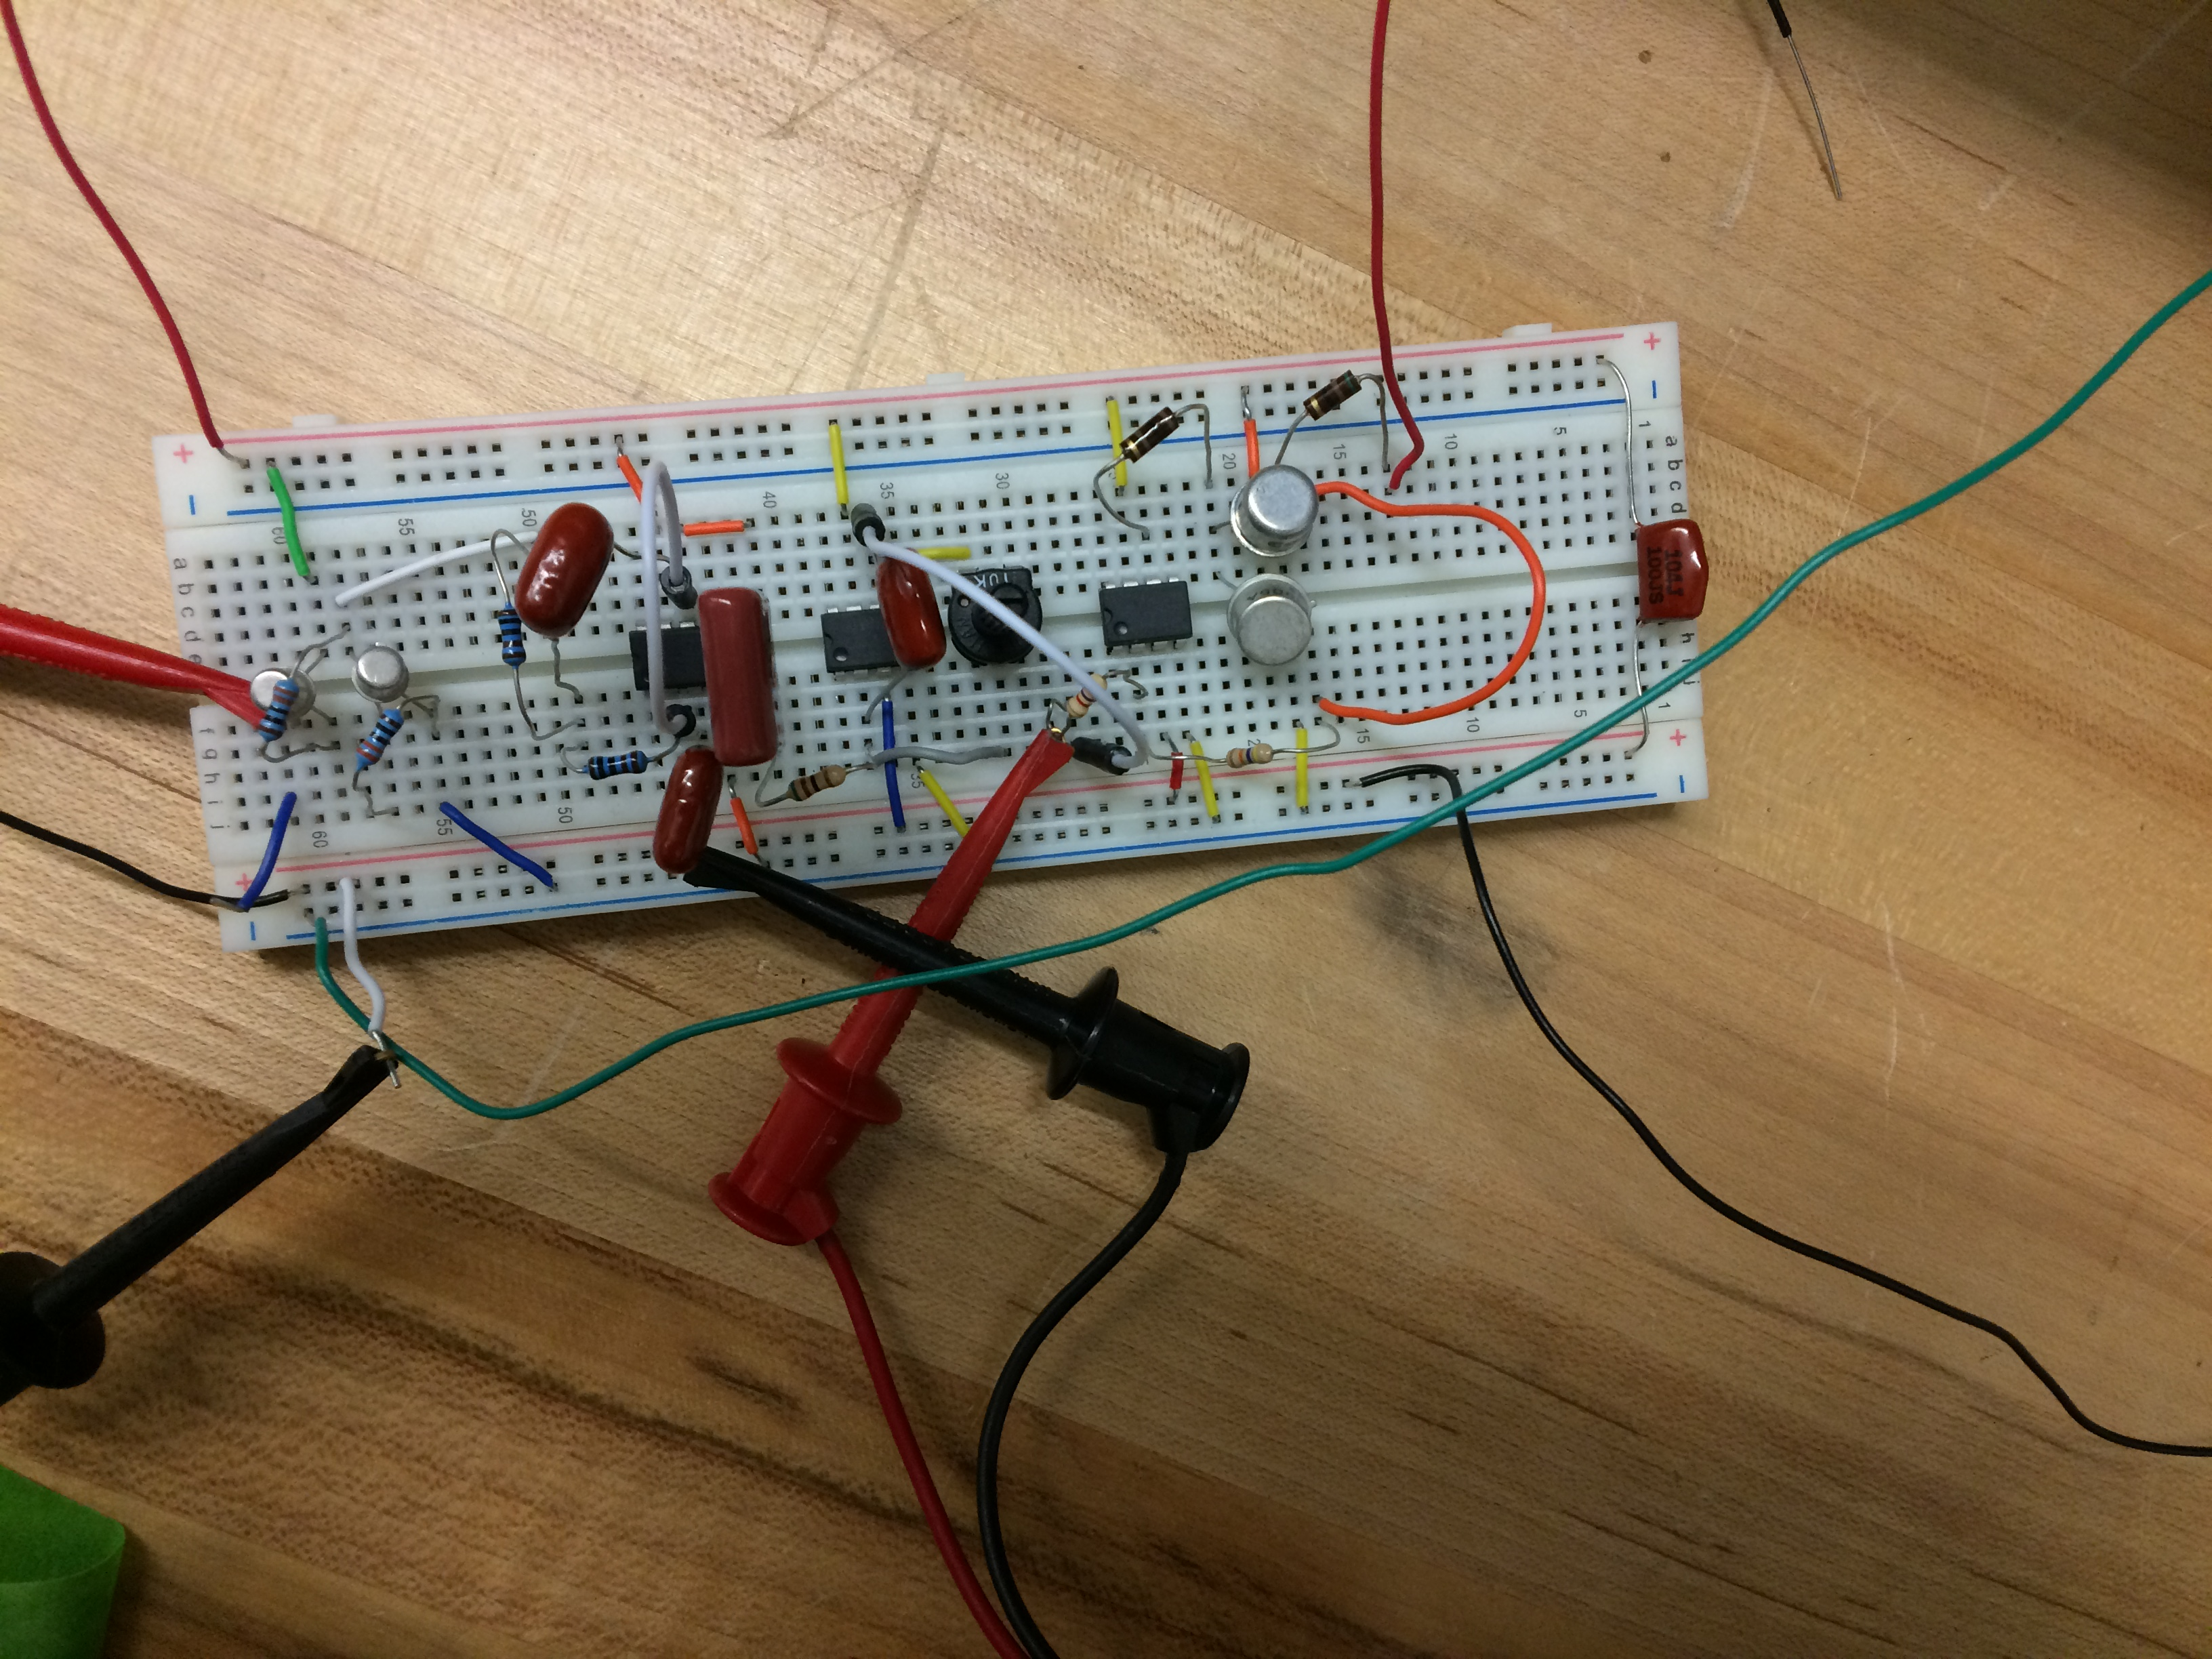
\includegraphics[scale = 0.07]{Auto2.JPG}
        \caption{Top view of actual circuit, not including piezo electric}
        \label{fig:my_label}
    \end{figure}
    \begin{figure}[H]
        \centering
        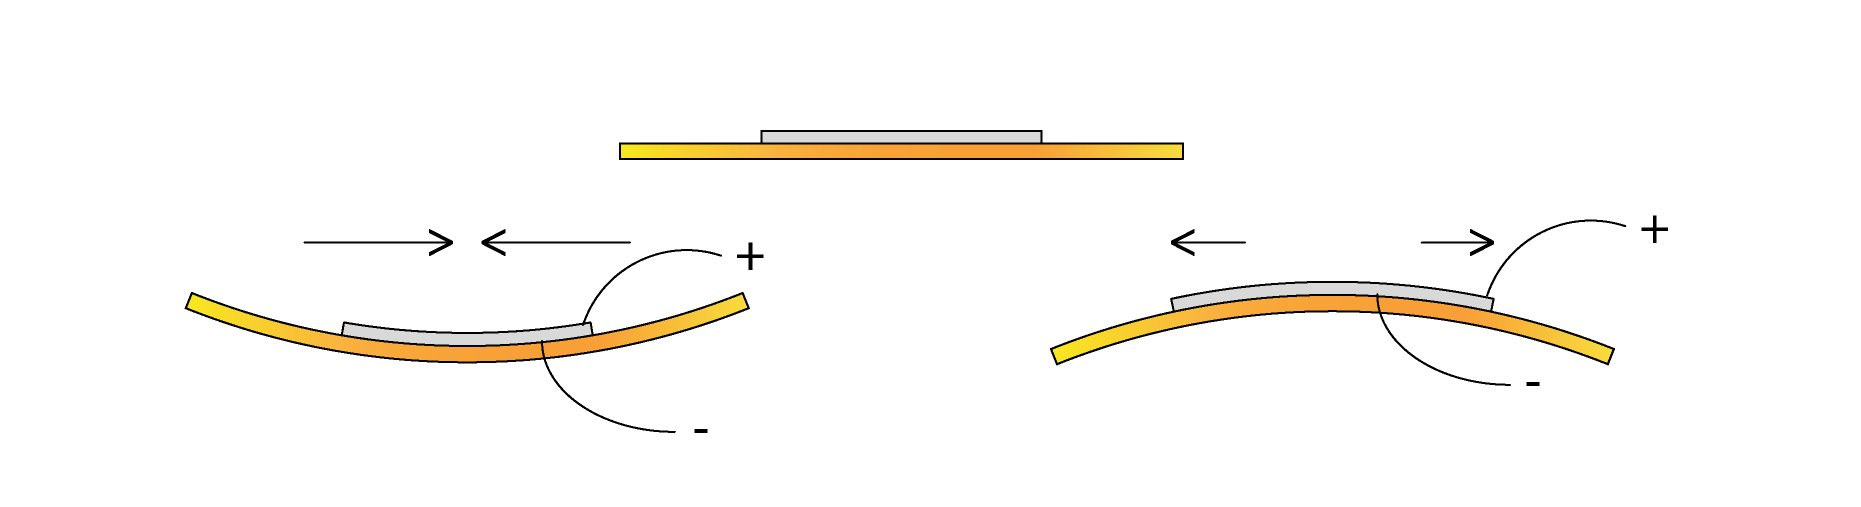
\includegraphics[scale = 0.5]{Piezo_bending_principle.jpg}
        \caption{Visual description showing piezo electric element undergoing tensile stress via mechanical vibrations, yielding voltage output from the device; ceramic piece is on top, brass at bottom \cite{wiki2}}
        \label{fig:my_label}
    \end{figure}
    \begin{figure}[H]
        \centering
        a)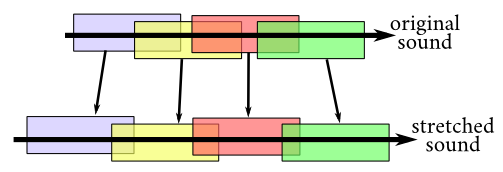
\includegraphics[scale=0.6]{stretchsound.png}
        b)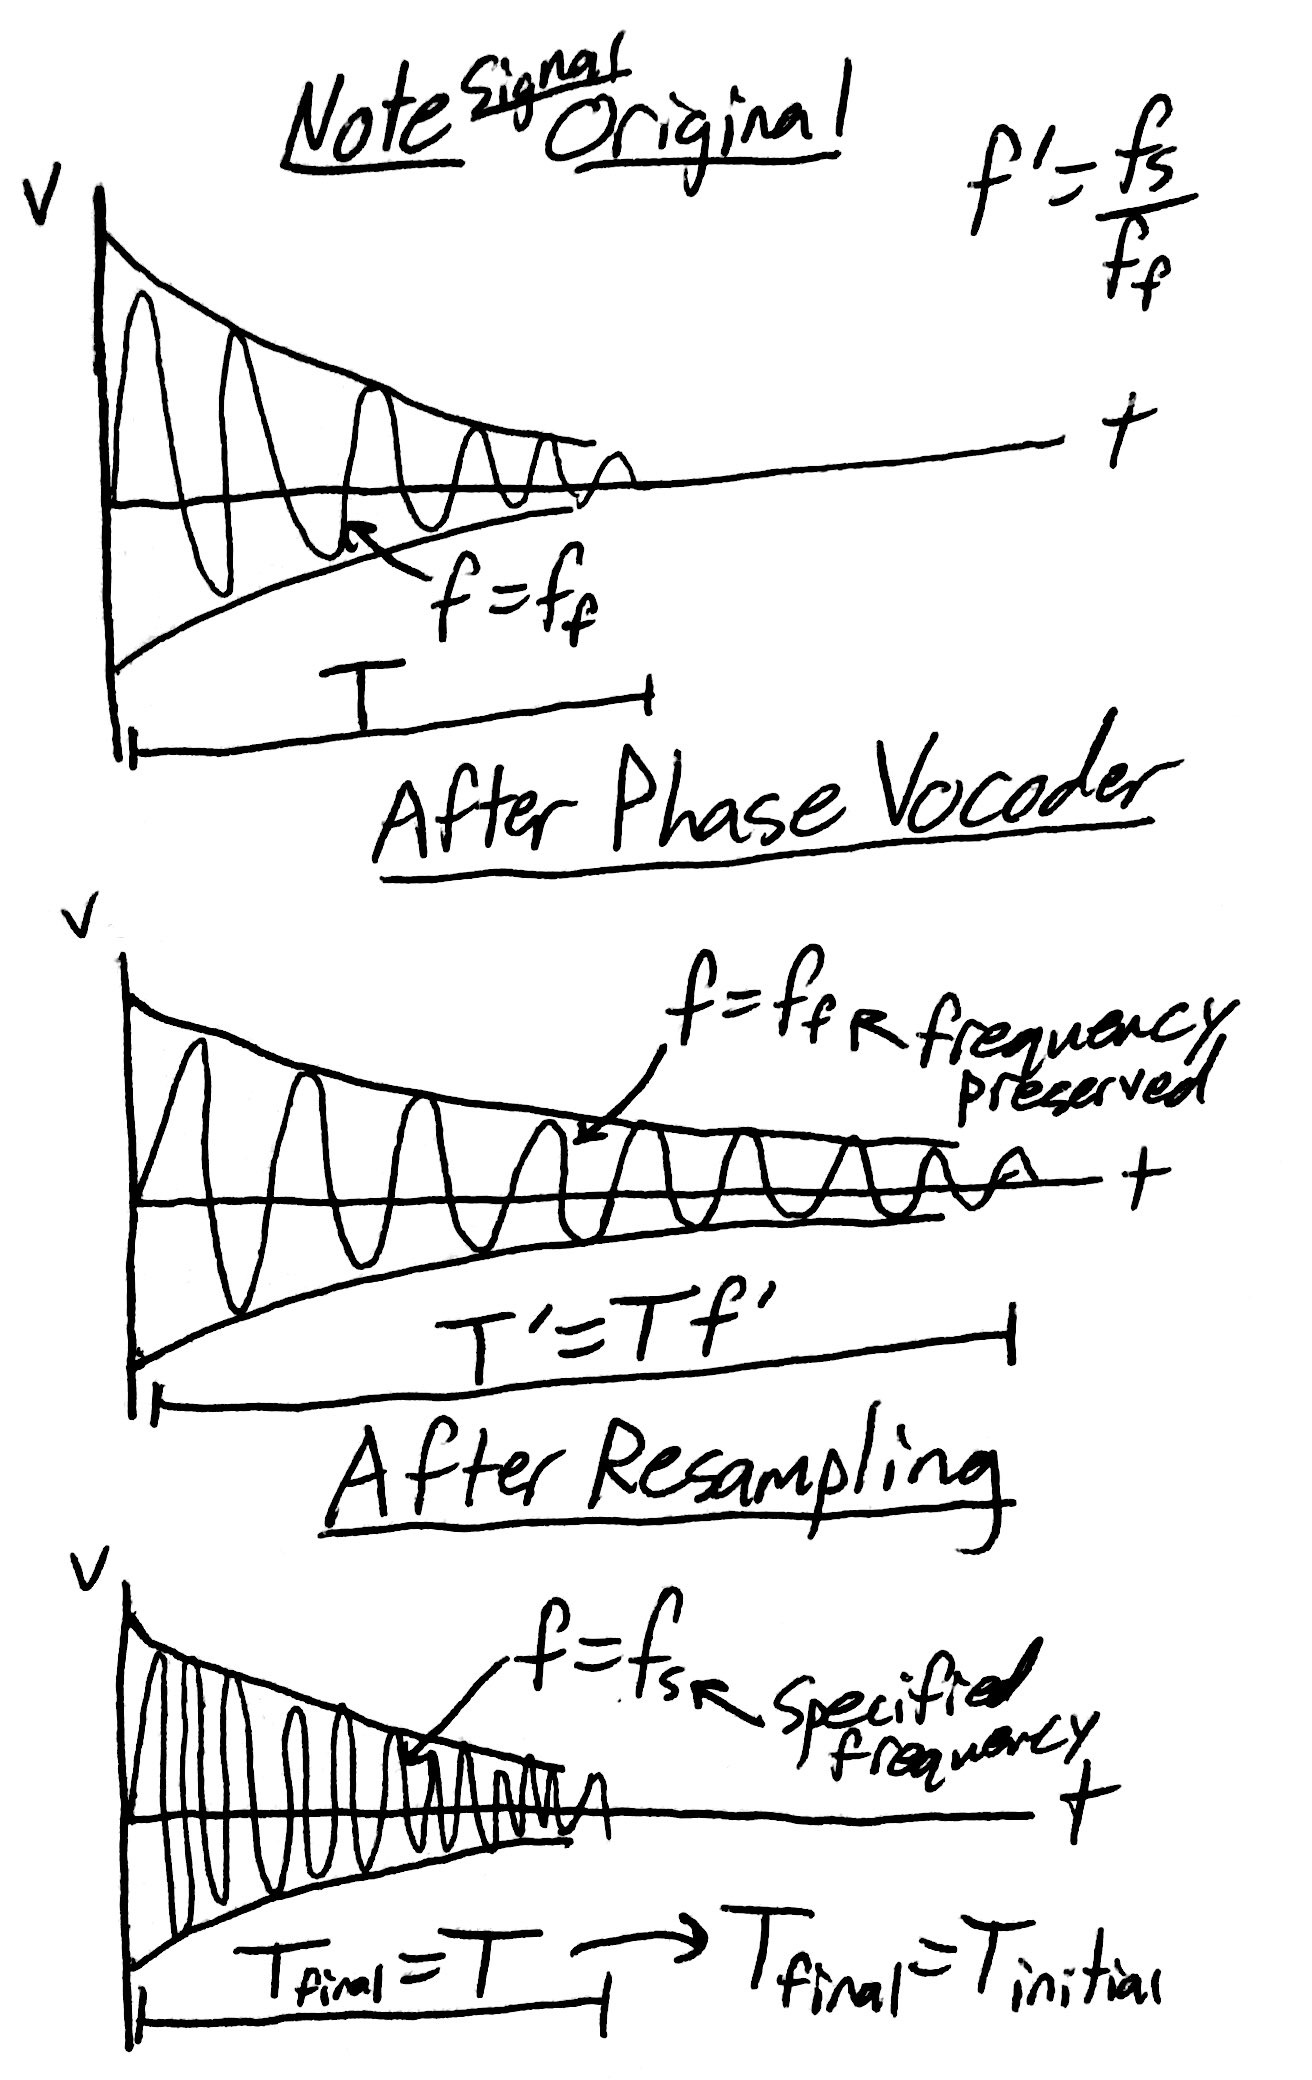
\includegraphics[scale = 0.12]{SongShifterMethod.jpg}
        c)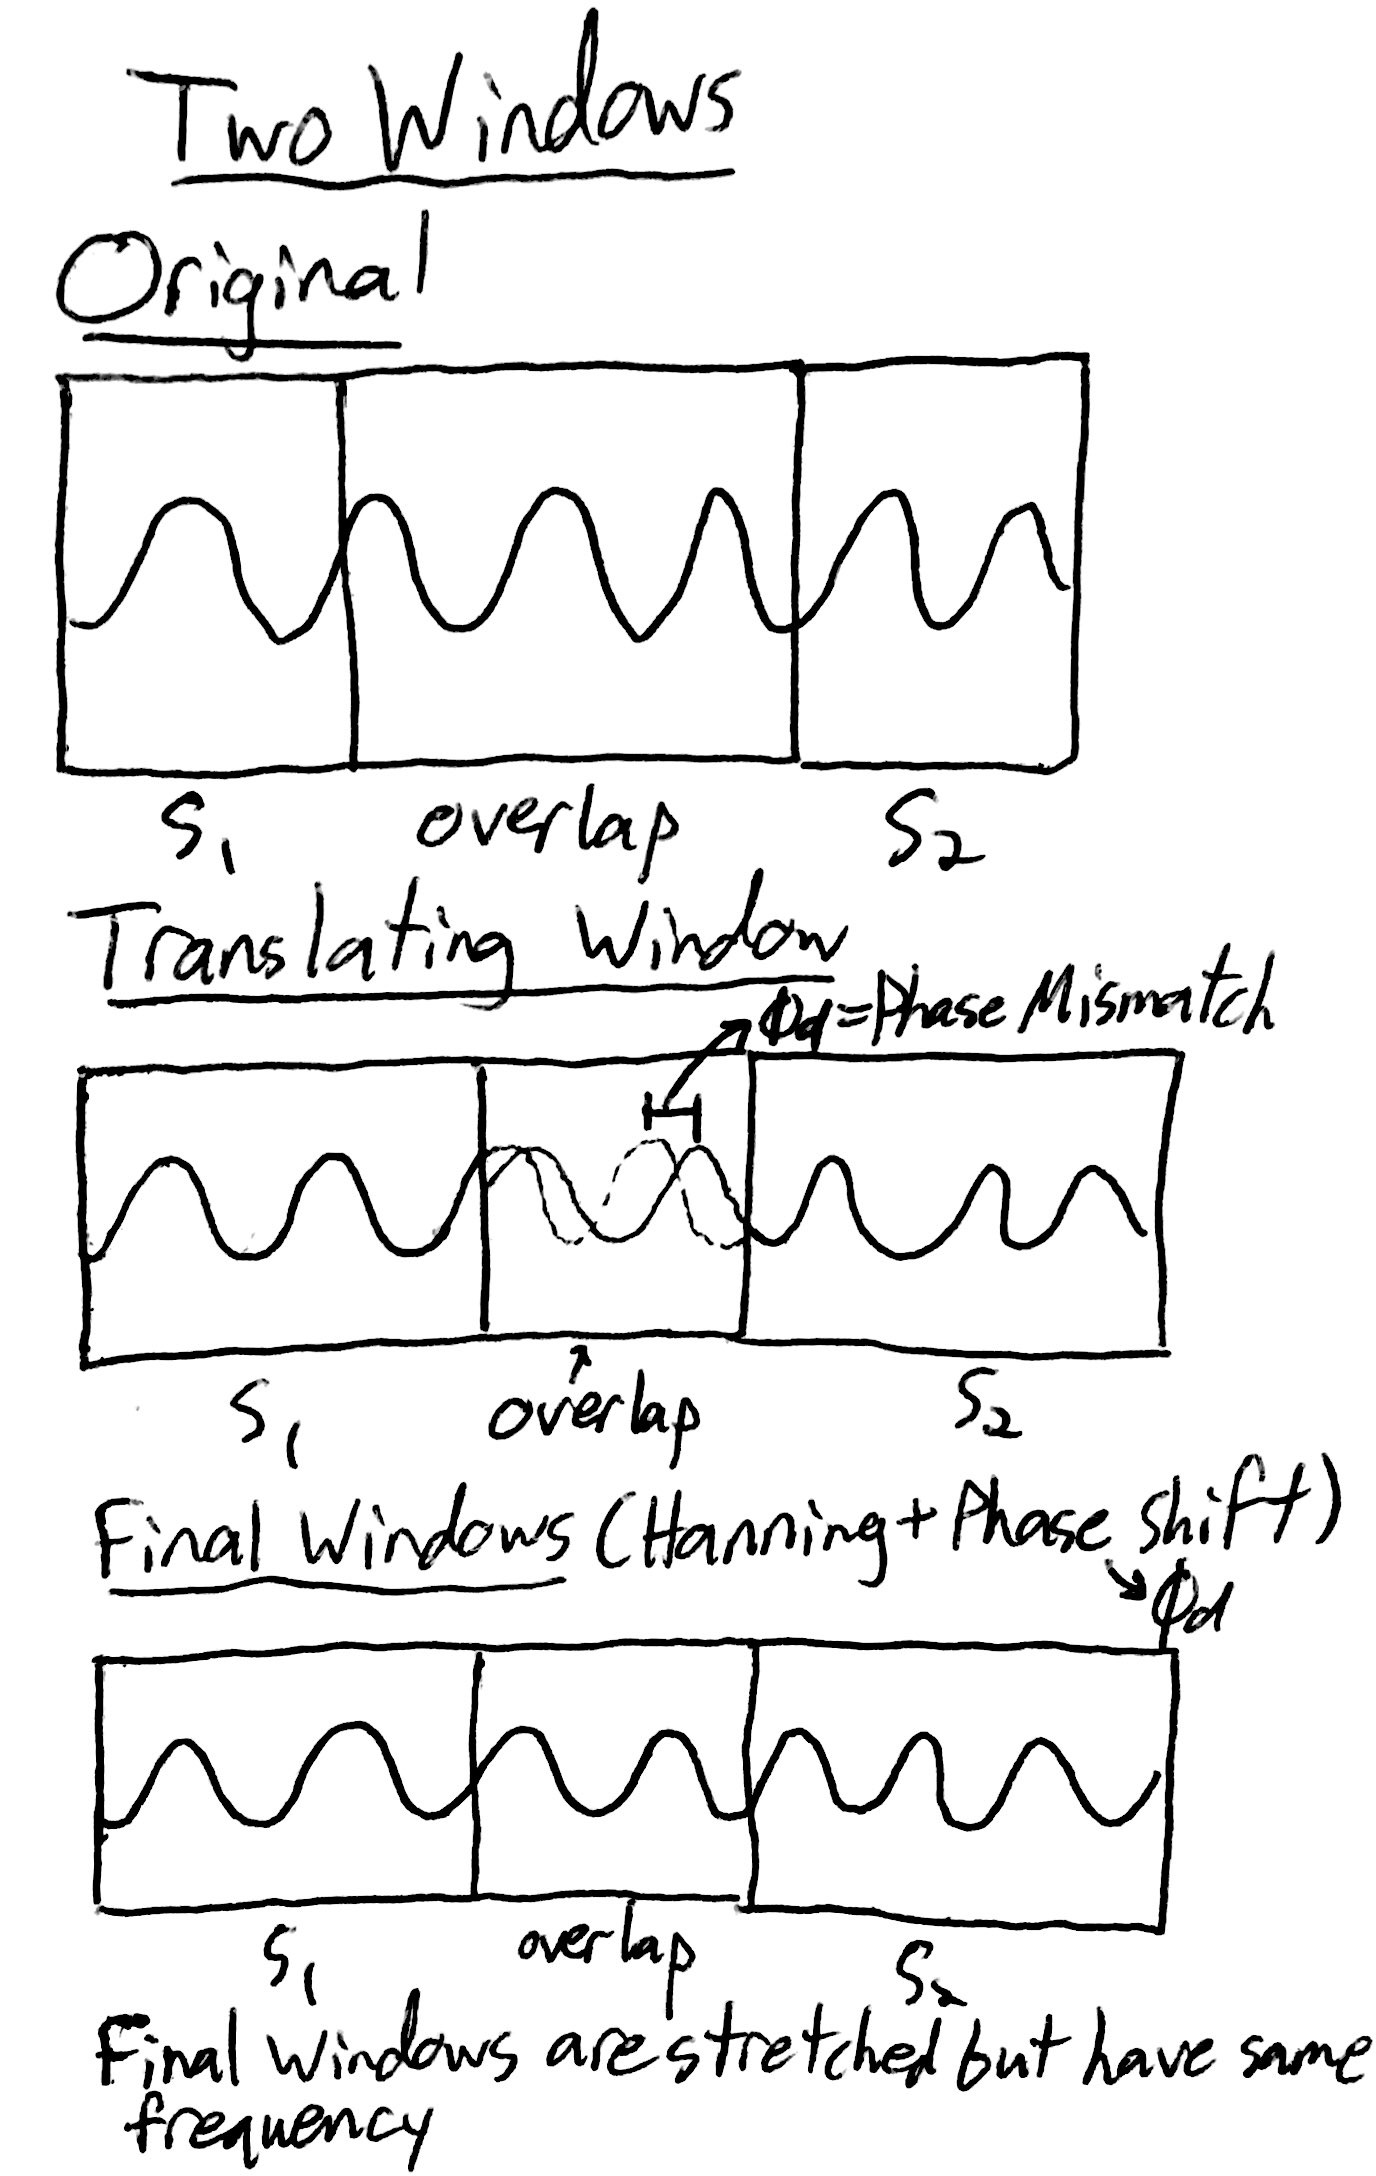
\includegraphics[scale = 0.12]{TwoWindows.jpg}
        \caption{Phase Vocoder/"Song Shifter": a) Break note into overlapping windows and horizontally translate windows to stretch/compress signal in time-domain with same frequency information \cite{phase}; b) Original note undergoing phase vocoder method, then being resampled to retain the original total time but with new specified frequency; c) Phase matching between two overlapping windows undergoing phase vocoder method, $S_2$ in final windows is the transformed $a_2$, to be added to the right of $S_1$, the sum of all overlapping windows forms phase vocoded note.}
        \label{fig:my_label}
    \end{figure}
    \begin{figure}[H]
            \centering
            a)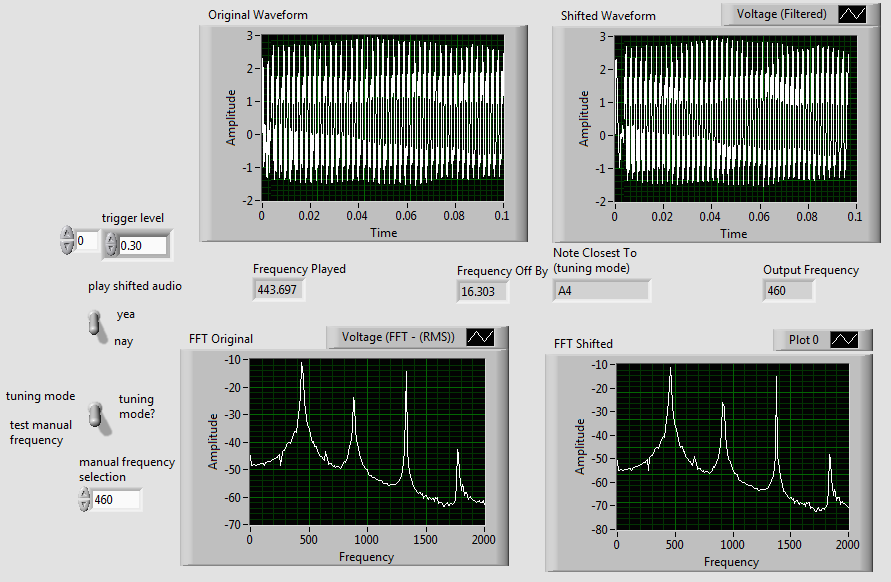
\includegraphics[scale=0.4]{front1.png}
            b)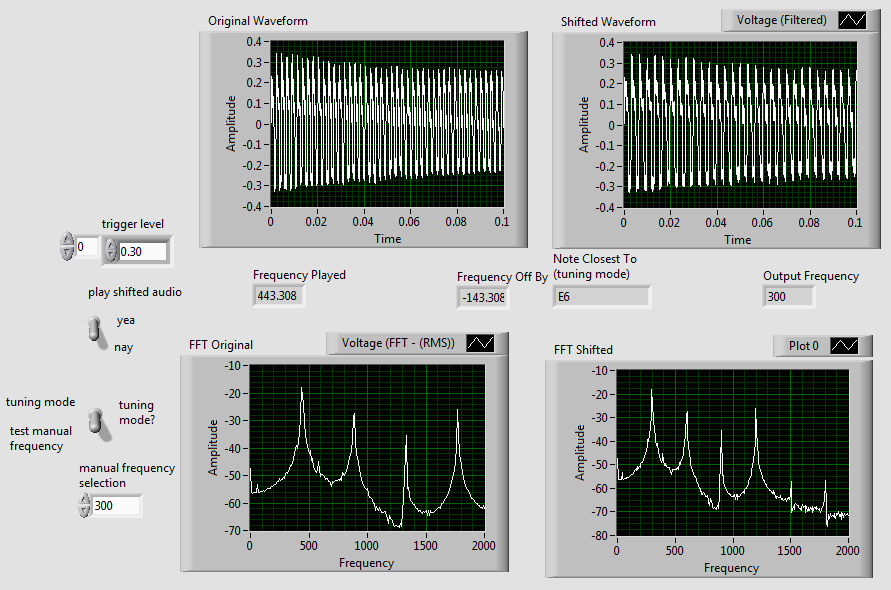
\includegraphics[scale=0.4]{front2.png}
            c)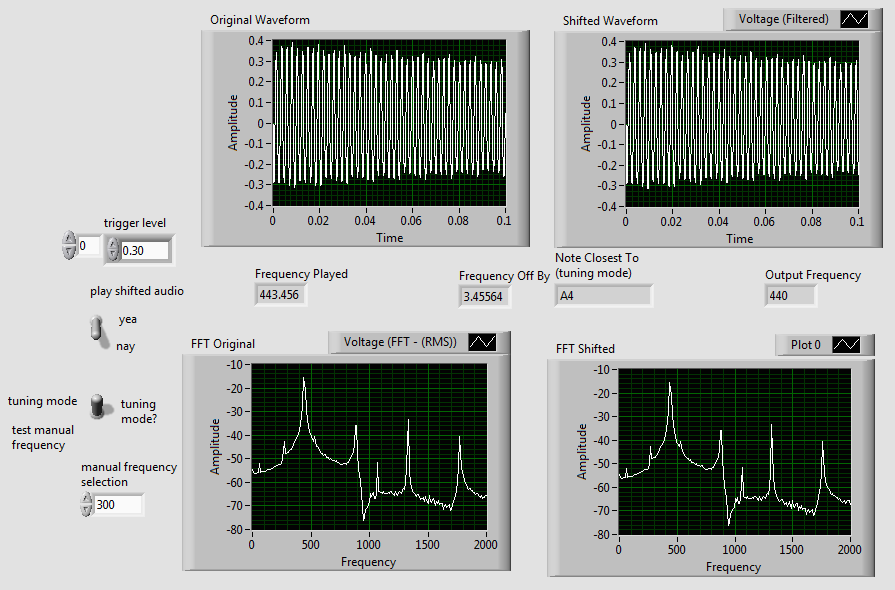
\includegraphics[scale=0.4]{front3.png}
            \caption{Three outputs of the front panels from the "Real-Time" method with the various options specified and a note of 443 Hz being played: a) Test manual frequency turned on and $f_s$ was set to 460Hz; b) Test manual frequency with $f_s = 300$Hz; and c) Tuning mode on, shifting to the closest note on the musical scale (A4, $f_s = 440$Hz)}
            \label{fig:my_label}
        \end{figure}
    \begin{figure}[H]
        \centering
        a)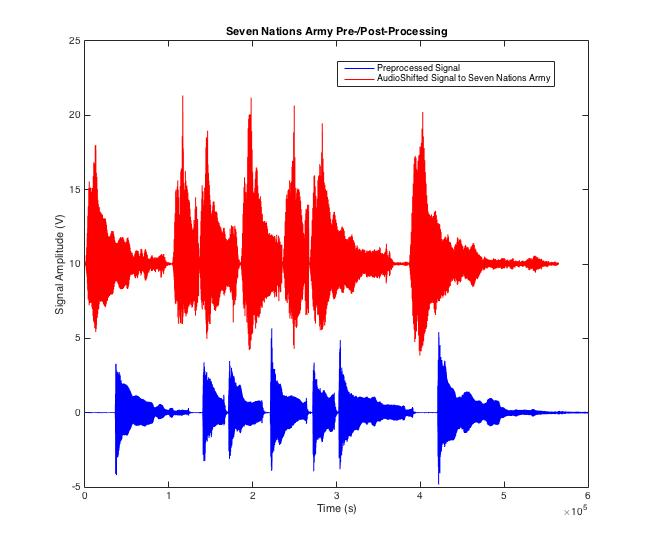
\includegraphics[scale=0.45]{SevenNationsArmyFigure.jpg}
        b)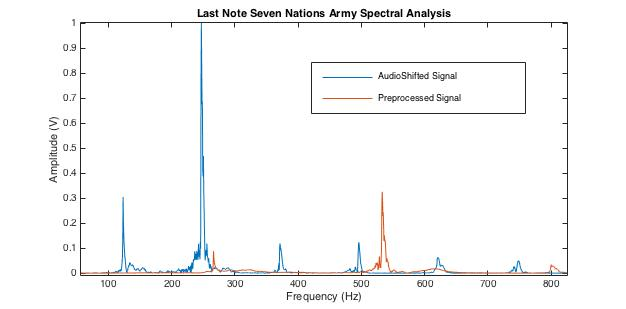
\includegraphics[scale = 0.45]{LastNote.jpg}
        c)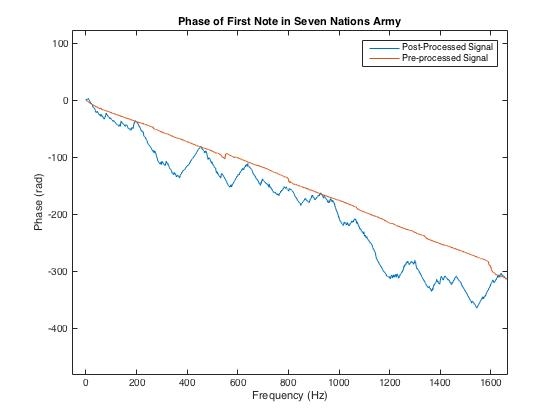
\includegraphics[scale = 0.45]{phaseProb.jpg}
        \caption{Comparisons of pre- to post processing of output from Song Shifter method, used to change 7 notes played at a frequency of 533 Hz to match the frequencies/notes of the song "Seven Nations Army": a) display of entire song signal, six second signal with post-processed translated 10V upwards; b) FFT of pre and post-processed/AudioShifted signal for last note; and c) phase information of first note}
        \label{fig:my_label}
    \end{figure}

\end{document}

